\documentclass[11pt, twocolumn]{article}

\usepackage[utf8]{inputenc}
\usepackage{graphicx}
\usepackage{amsmath}
\usepackage[a4paper, total={7in, 9in}]{geometry}


\title{Probability Cheatsheet}
\author{Yahya~Almardeny\\almardeny@gmail.com}
\date{June 2019}

\begin{document}
\begin{titlepage}
\maketitle
\end{titlepage}

\section{Overview}
Probability provides measures for reasoning the likelihood that an event will occur in an experiment.
\section{Terminology}
\begin{enumerate}
\item \textbf{Experiment}: Procedure that yields one of the possible outcomes. E.g. Tossing a coin.
\item \textbf{Sample Space S}: A set of all possible outcomes of an experiment. E.g. S = \{Head, Tail\} when tossing a fair coin.
\item \textbf{Event E}: Set of outcomes of an experiment. Note that if the Event contains only one outcome, it is then called an elementary event. E.g. The event that coin is Head.
\end{enumerate}
\section{Random Variable R.V}
A variable that its possible values are the outcomes of an experiment. It has two types:
\begin{enumerate}
\item \textbf{Discrete R.V}: Take one countable number of distinct values. E.g 1, 2, 3, 4
\item \textbf{Continuous R.V}: Take infinite number of possible values (usually measurements). E.g. all interval values in the range [1 - 2].
\end{enumerate}

\section{Probability of Events}
\begin{enumerate}
\item \textbf{Marginal probability}: Simply $P(A)$ which means "unconditional probability". And for each outcome $s$, it should satisfy: $ 0 \leq P(s) \leq 1$ and $\Sigma P(s_i) = 1$.
\item \textbf{Addition Rule}: $P(A \cup B) = P(A) + P(B) - P(A \cap B)$ where $\cup$ means OR, $\cap$ means AND.
\item \textbf{Joint (Compound) Probability Rule}:
	\begin{enumerate}
	\item Independent Events: $P(A \cap B) = P(A) \times P(B)$.
	\item Dependent Events: $P(A \cap B) = P(A) \times P(B | A)$. where $P(B | A)$ read: Probability of B given A had happened.
	\end{enumerate}
\item \textbf{Conditional Probability}: $P(A | B) = \frac{P(A \cap B)}{P(B)}$
\item \textbf{Bayes Theorem}: $P(A | B) = \frac{P(B | A) \times P(A)}{P(B)}$. It gives the probability of A based on prior knowledge of B.
\end{enumerate}

\section{Probability Distributions}
\begin{enumerate}
\item \textbf{Probability Mass Function (PMF)}: Gives the probability a \textit{discrete} R.V $X$ takes on the value $x$: $P( X = x)$.
\begin{figure}[h!]
  \centering
  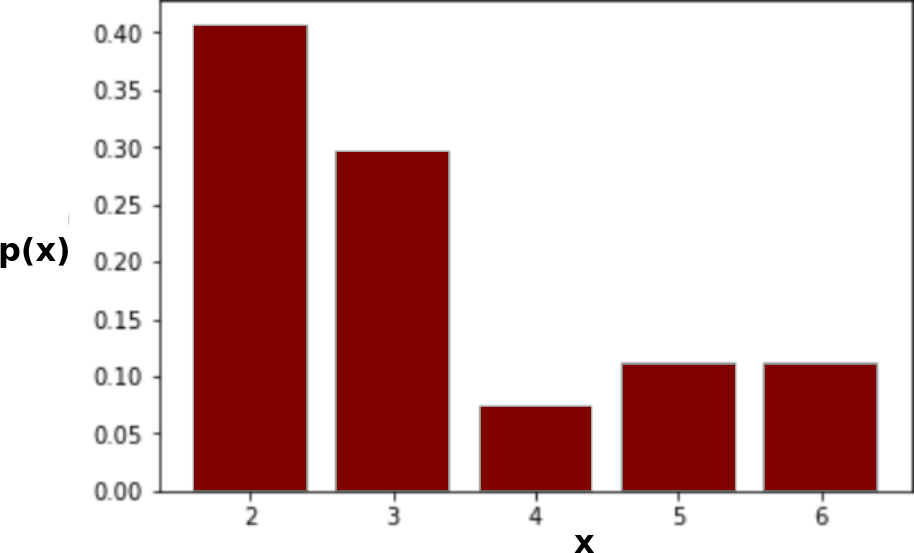
\includegraphics[width=0.7\linewidth]{figs/PMF.png}
\end{figure}
\item \textbf{Probability Density Function (PDF)}: Gives the probability a \textit{continuous} R.V $X$ takes on the value $x$: $P( X = x)$ which means how dense the probability of $X$ near $x$, and it will be the definite Integrals between two points.
\begin{figure}[h!]
  \centering
  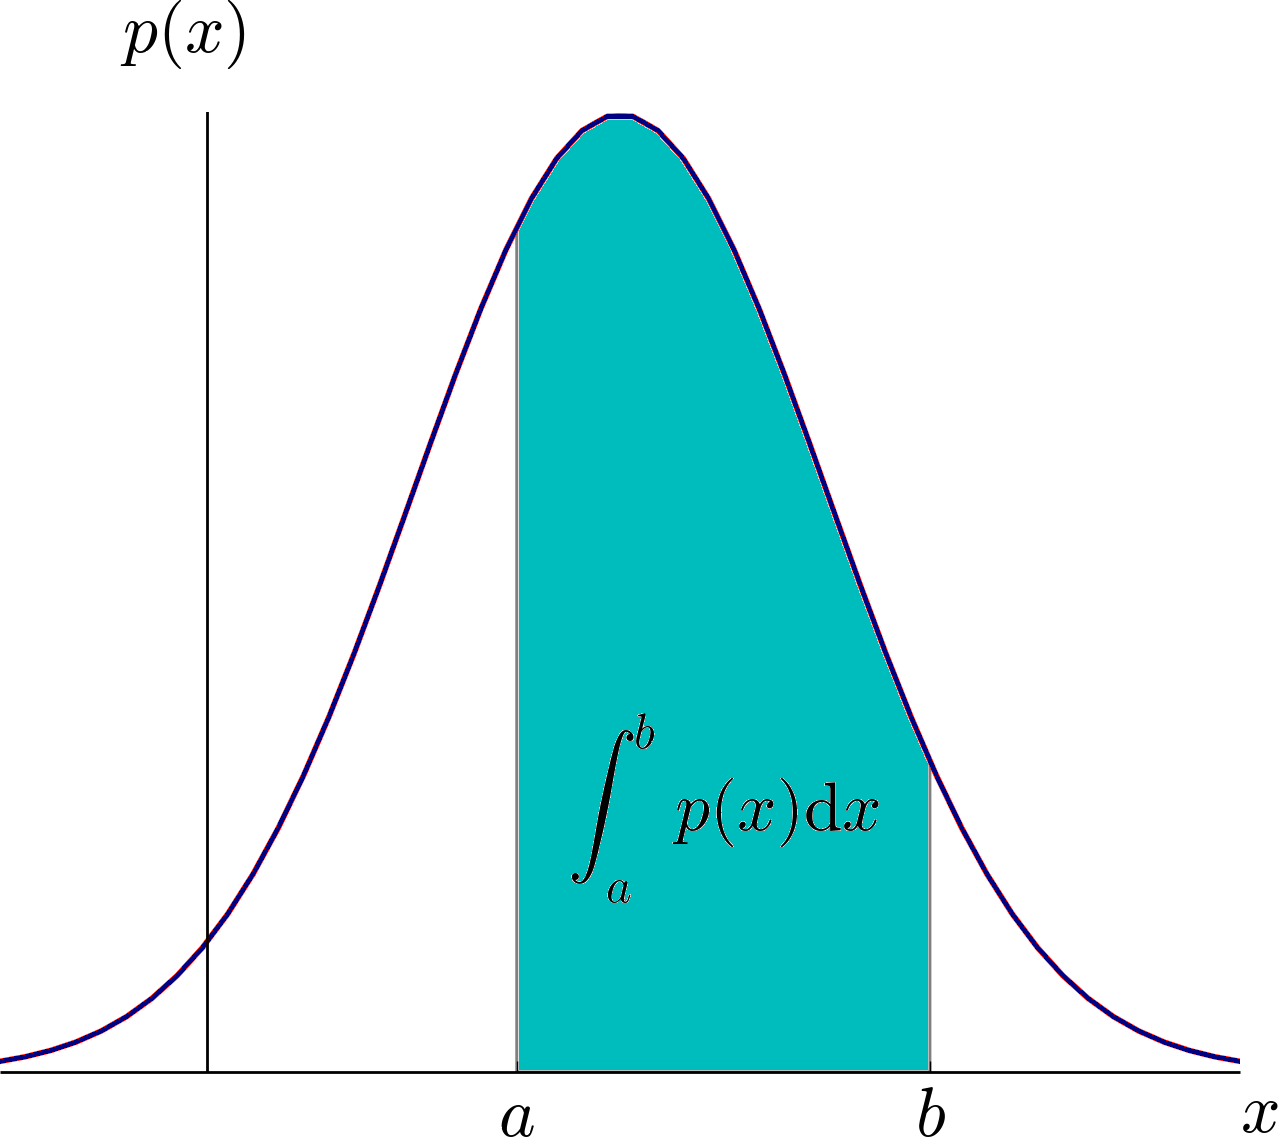
\includegraphics[width=0.6\linewidth]{figs/PDF.png}
\end{figure}
\item \textbf{Cumulative Density Function (CDF)}: Gives the probability a R.V $X$ is less than or equals the value $x$: $P( X \leq x)$. It is  cumulative because it adds the probabilities up to $x$.
	\begin{enumerate}
	\item For Discrete R.V: It is the summation of previous probabilities $\Sigma p(x_i)$.
	\item For Continuous R.V: It is the integral $\int_{-\infty}^{x} p(x) dx$
	\end{enumerate}
\end{enumerate}

\section{Expected Value of R.V}
Intuitively, it is the long-run average value of repetitions of the same experiment it represents (i.e. what outcome to expect on long run)
\begin{enumerate}
\item \textbf{For a Discrete R.V}: It is the average of R.V values based on their associated probabilities $E(X) = \Sigma (x_i \times p(x_i))$.
\item \textbf{For a Continuous R.V}: $E(X) = \int_{-\infty}^{\infty} x f(x) dx$ where $f(x)$ is probability density function.
\end{enumerate}

\section{Combining Random Variables}
If we have two independent random variables $X$ and $Y$, we can add or subtract to get the total or the difference of their means (expected values) and variances:
$T = X \pm Y \Rightarrow \mu_T = \mu_X \pm \mu_Y  ~~ and ~~ \sigma_T^2 = \sigma_X^2 \pm \sigma_Y^2$.

\section{The Law of Large Numbers}
Let $X$ be R.V of a population where its expected value (i.e Mean) is $E(X)$. Let $\overline{X_n} = \frac{x_1 + x_2 + ... x_n}{n}$ be the mean of $n$ samples $\in X$. As $n \to \infty$ : $\overline{X_n} \to E(X)$. Which means as we do more experiments, the outcomes become closer and closer to the outcomes of the probability theory.

\section{Statistical Distributions}\footnote{Included because it is related directly to probability}
\begin{enumerate}
\item \textbf{Binomial Distribution}: How many success in finite number of trials:
	\begin{itemize}
	\item Made up of \textit{independent} trials.
	\item Each trial has one of two \textit{discrete} outcomes (success or failure).
	\item \textit{Fixed} number of trials
	\item Probability of success in each trial is \textit{constant}.
	\item E.g. X = number of heads after 10 flips of a coin.	
	\item \textit{10\% Rule}: We assume independence if the sample $\leq$ 10\% of the population.
	\item PMF: $P(X = x) = (_{n}^{k}) p^x (1 - p)^{n-x}$ which means the probability of $k$ successes in $n$ trials.
	\item $E(X) = \mu_X = n . p$ where $p$ is the probability of success per trial.
	\item $\sigma_X = \sqrt{var(X)} = \sqrt{n . p (1 - p)}$.
	\item The more trials we do, the more Binomial becomes Normal distribution.
	\end{itemize} 

\item \textbf{Bernoulli Distribution}: Simply a Binomial Distribution with just \textit{one} trial. 
\item \textbf{Geometric Distribution}: How many trials until success?. It is similar to Binomial dist. but here we do not have fixed number of trials because we do not know ahead how many trials until we get the desired outcome:
	\begin{itemize}
	\item PMF: $P(X = x) = (1 - p)^{k - 1} p$.
	\item $E(X) = \mu_X = \frac{1}{p}$.
	\item $\sigma_X = \sqrt{var(X)} = \sqrt{\frac{1 - p}{p^2}}$.
	\end{itemize} 

\item \textbf{Hypergeometric Distribution}: It is a \textit{discrete} probability distribution that describes the probability of $k$ successes in $n$ draws, \textit{without} replacement, from a finite population of size $N$ that contains exactly $K$ objects. In contrast, the binomial distribution describes the probability of $k$ successes in $n$ draws \textit{with} replacement. 
	
\item \textbf{Poisson Distribution}: It is a \textit{discrete} probability distribution that predicts \textit{rare} events that are independent of one another and occur with a known constant rate $\lambda$. It is usually used instead of Binomial dist. if the number of trials is very high (fixed interval of time) and the probability (occurrence) of each is relatively low:
	\begin{itemize}
	\item PMF: $P\left( x \right) = \frac{{\lambda ^x }}{{x!}} e^{ - \lambda } $.
	\item Mean is $E(X) = \lambda$. and Variance is $\lambda$.
	\end{itemize} 

\item \textbf{Normal Distribution (a.k.a Gaussian)}: It is a \textit{continuous} probability distribution that has the notation  $X \sim \mathcal{N}(\mu,\,\sigma^{2})$. It is symmetric and has a bell shape where most of the values are near to the mean and follows the 68–95–99.7 rule (a.k.a empirical rule). This rule states that 68.27\%, 95.45\% and 99.73\% of the values lie within one, two and three standard deviations of the mean, respectively:
	\begin{itemize}
	\item PDF: $P(x) = \frac{1}{{\sigma \sqrt {2\pi } }}e^{{{ - \left( {x - \mu } \right)^2 } \mathord{\left/ {\vphantom {{ - \left( {x - \mu } \right)^2 } {2\sigma ^2 }}} \right. \kern-\nulldelimiterspace} {2\sigma ^2 }}}$.
	\item Mean is $E(X) = \mu_X$. and Variance is $\sigma_X^2$.
	\end{itemize} 
	
\item \textbf{Log-Normal Distribution}: It is a \textit{continuous} probability distribution of a random variable whose \textit{logarithm is normally distributed}.Because the values in a log-normal distribution are positive, they create a right-skewed curve which is important in determining which distribution is appropriate to use in investment decision-making.  One of the most common applications of log-normal distributions is in the analysis of stock prices. A log-normal distribution can be translated to a normal distribution and vice versa using associated logarithmic calculations.
	
\item \textbf{Uniform Distribution}: It is a probability distribution that has \textit{constant} probability. 
	\begin{enumerate}
	\item \textit{Discrete Uniform Dist.}:  It takes one of a finite $n$ possible values:
		\begin{itemize}
		\item PMF: $P(X = x) = \frac{1}{n}$
		\item $E(X) = \mu_X = \frac{(a + b)}{2}$
		\item $\sigma_X^2 =\frac{(b - a + 1)^2 ~ - 1 }{12}$
		\end{itemize} 

	\item \textit{Continuous Uniform Dist.}: It takes values within a specified range $a$ to $b$:
		\begin{itemize}
		\item PDF:
		\begin{align*}
			P(X = x) = \begin{cases}  \frac{1}{b-a}~ if ~ x \in [a , b]\\ 0 ~ otherwise \end{cases}
		\end{align*}
		\item $E(X) = \mu_X = \frac{1}{2} (a+b)$
		\item $\sigma_X^2 =\frac{1}{12} (b - a)^2 $
		\end{itemize} 

	\end{enumerate}

\item \textbf{Gamma Distribution}: It is a family of a \textit{continuous}, \textit{positive-only}, \textit{unimodal} distributions that encode the time required for $alpha$ events to occur in a Poisson process with mean arrival time of $beta$. These distributions are useful in real-life where something has a natural minimum of $0$. For example, it is commonly used in finance, for elapsed times, or during Poisson processes. In other words, it is a generalization of both the exponential and chi-squared distributions.
		
\item \textbf{Exponential Distribution}: Special case of Gamma Distribution. It is a \textit{continuous} analogue of the geometric distribution and often used to model the time elapsed between events. Formally, it is the probability distribution of the time between events in a process where events occur continuously and independently at a \textit{constant} average rate (i.e. Poisson process):
		\begin{itemize}
		\item PDF: $P(X = x) = {\lambda e}^{-\lambda x}$
		\item $E(X) = \mu_X = \lambda^{-1} = \beta$
		\item $\sigma_X^2 =\lambda^{-2} = \beta^2$
		\end{itemize} 

\item \textbf{Chi-Square Distribution}:  It is a special case of the Gamma distribution. It is a \textit{continuous} distribution of a sum of the squares of $k$ independent standard normal deviates (where $k$ is known as degree of freedom).  A standard normal deviate is a \textit{random sample} from the standard normal distribution.
		\begin{itemize}
		\item PDF: $P(X = x) = {\frac{1}{2^{\frac{k}{2}}\Gamma(	\frac{K}{2})}}^{x^{\frac{k}{2}-1}~e^{\frac{-x}{2}}}$ where $\Gamma$ is the gamma function
		\item $E(X) = \mu_X = k$
		\item $\sigma_X^2 = 2k$
		\end{itemize} 
	
\item \textbf{Student's t-Distribution}:  It is a probability distribution used to estimate population parameters when the sample size is small and standard deviation is unknown. It is mainly used by applying Student's t-test for assessing the statistical significance of the difference between two sample means, and in linear regression analysis. 
		\begin{itemize}
		\item PDF: $$ \frac{\Gamma (\frac{\nu+1}{2})}{\sqrt{\nu \pi} \Gamma (\frac{\nu}{2})} (1 + \frac{x^2}{\nu})^{-\frac{\nu+1}{2}}
$$ where $\nu$ is the number of degrees of freedom and $\Gamma$ is the gamma function.
		\item $E(X) = \mu_X = 	0 ~ for ~ \nu > 1,$ otherwise undefined.
		\item $\sigma_X^2 = \frac{\nu }{\nu -2} ~for~ \nu >2, ~\infty ~for~ 1 < \nu \le 2,$ otherwise undefined.
		\end{itemize} 
\end{enumerate}

\end{document}






